\chapter{Technical Background}
\label{chapter:background}

This chapter establishes the scientific foundation for the screening system: it defines \ab{mtbi} and the pathology that resists conventional imaging (\Cref{sec:bg-mtbi}), evaluates existing diagnostic approaches against the screening requirements of \Cref{chapter:introduction} to motivate automated oculomotor screening (\Cref{sec:bg-existing}), details the oculomotor biomarkers underpinning the design (\Cref{sec:bg-oculomotor}), and surveys prior engineering work (\Cref{sec:bg-engineering}).

\section{Mild Traumatic Brain Injury}
\label{sec:bg-mtbi}

\ab{mtbi}, also known as concussion, is defined by the 2023 American Congress of Rehabilitation Medicine criteria as traumatic brain injury with a \ab{gcs} score of 13--15, loss of consciousness lasting less than 30 minutes, and post-traumatic amnesia persisting for less than 24 hours~\cite{silverberg2023acrm}. These thresholds distinguish mild from moderate (\ab{gcs} 9--12) and severe (\ab{gcs} 3--8) TBI. Importantly, the term ``mild'' refers to the initial injury severity classification, not the clinical outcome: a substantial minority of patients experience persistent symptoms and significant disability despite classification as mild~\cite{silverberg2023acrm}.

A primary pathological feature of \ab{mtbi} is \ab{dai}, in which rapid acceleration-deceleration and rotational forces during impact cause widespread microscopic damage to axons~\cite{johnson2013axonal}. Shear forces disrupt axonal microtubules, particularly in white matter tracts such as the corpus callosum, internal capsule, and cerebellar peduncles. This occurs alongside a broader neurometabolic cascade involving ionic flux, excitotoxicity, and neuroinflammation. Unlike focal contusions, \ab{dai} is typically invisible on conventional CT and MRI~\cite{lee2005neuroimaging, palacios2022dti}, motivating screening approaches that do not rely on structural imaging.


\section{Existing Diagnostic Approaches}
\label{sec:bg-existing}

\begin{figure}[b]
    \centering
    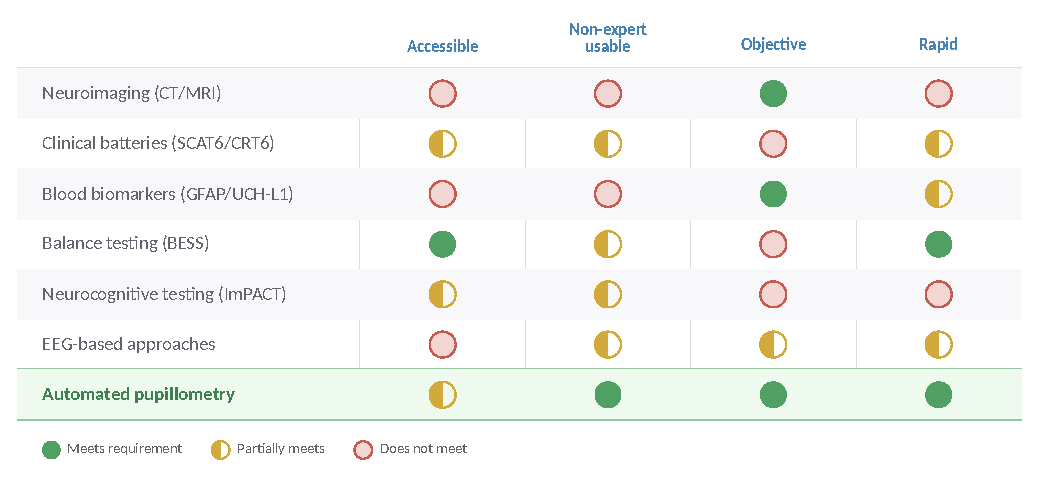
\includegraphics[width=\textwidth]{figures/screening_comparison.pdf}
    \caption{Comparison of candidate mTBI screening approaches against the four requirements identified in \Cref{chapter:introduction}. Automated oculomotor screening most closely satisfies all four criteria, though most existing commercial implementations remain expensive and clinic-based. This accessibility gap is the engineering problem addressed by this project.}
    \label{fig:screening_comparison}
\end{figure}

This section evaluates existing diagnostic approaches against the four requirements of \Cref{chapter:introduction} (\Cref{fig:screening_comparison}) to motivate the choice of automated oculomotor screening.

\textbf{Neuroimaging.} Neuroimaging serves a different clinical purpose to field screening: CT and MRI are used to rule out life-threatening pathology such as intracranial haemorrhage once a patient has reached hospital, not to diagnose \ab{mtbi} at the point of injury~\cite{stiell2001ct, haydel2000ct}. MRI detects abnormalities in approximately 28\% of CT-negative patients~\cite{yuh2013mri}, but most \ab{mtbi} cases remain invisible even on MRI. Advanced diffusion tensor imaging can detect white matter microstructural changes~\cite{palacios2022dti} but remains a research tool. All neuroimaging modalities require hospital infrastructure, specialist operation, and substantial cost.

\textbf{Clinical assessment batteries.} The \ab{scat6} provides structured evaluation combining symptom inventories, cognitive screening, and balance testing, but requires a trained healthcare professional to administer and interpret~\cite{echemendia2023scat6}. The CRT6, designed for non-medical personnel, provides only observational guidance without quantitative metrics~\cite{echemendia2023crt6}. Systematic reviews report highly variable diagnostic performance across assessment components, with sensitivity ranging from 13--92\%~\cite{nelson2013diagnostic}. All such tools depend on either medical training or patient self-report, the latter being vulnerable to symptom minimisation by athletes motivated to continue playing~\cite{meier2015underreporting}.

\textbf{Blood biomarkers.} The FDA-cleared combination of GFAP and UCH-L1 serum biomarkers achieved 97.5\% sensitivity for predicting CT-visible abnormalities, but only approximately 40\% specificity~\cite{bazarian2018blood}. Importantly, these biomarkers are validated for predicting CT findings, not for diagnosing \ab{mtbi} itself. They require venipuncture by trained personnel, laboratory or point-of-care analyser infrastructure, and must be collected within 12 hours of injury. These constraints preclude field deployment by non-medical personnel.

\textbf{Balance and neurocognitive testing.} The Balance Error Scoring System (BESS), commonly used alongside the \ab{scat6}, demonstrates poor sensitivity of only 34\% acutely, declining further over subsequent days~\cite{bell2011bess}. Computerised neurocognitive tests such as ImPACT achieve higher sensitivity (approximately 82\%) but require baseline comparison testing, are vulnerable to deliberate underperformance, and take 20--25 minutes to administer~\cite{schatz2006impact}. Both approaches depend on patient cooperation and physical or cognitive effort.

\textbf{EEG-based approaches.} Quantitative EEG and event-related potential measurements can detect electrophysiological changes following \ab{mtbi}. However, the American Clinical Neurophysiology Society has stated that current evidence does not support the clinical use of quantitative EEG for diagnosing \ab{mtbi}~\cite{nuwer2021qeeg}. Portable systems exist but require electrode application and are sensitive to movement artefact in field environments.

\textbf{Automated oculomotor screening.} Quantitative measurement of the pupillary light reflex and other oculomotor responses provides objective, involuntary biomarkers that do not depend on patient self-report or cooperation. Automated systems require minimal training, can complete assessment in under one minute, and have demonstrated diagnostic accuracy of 91--96\% with machine learning analysis~\cite{maxin2024smartphone}. Automated oculomotor screening therefore satisfies three of the four screening requirements directly: usable by non-experts, objective and cooperation-independent, and rapid. However, most existing commercial systems cost thousands of pounds and are designed for clinical facilities, leaving accessibility as the unresolved engineering challenge this project addresses.

\textbf{Synthesis.} Automated oculomotor screening is the only reviewed approach that satisfies or partially satisfies all four screening requirements (\Cref{fig:screening_comparison}), with accessibility the remaining barrier. The highest published accuracy figures derive from machine learning models validated in specific cohorts, and prospective multi-site validation remains necessary.


\section{Oculomotor Biomarkers}
\label{sec:bg-oculomotor}

Oculomotor dysfunction is observed in 65--90\% of individuals following \ab{mtbi}~\cite{mcdonald2022eye}. This high prevalence reflects the vulnerability of brainstem and midbrain structures to diffuse axonal injury: the oculomotor nucleus, Edinger-Westphal nucleus, and mesencephalic reticular formation all lie in regions particularly susceptible to shearing forces during head acceleration~\cite{hirad2019neural}. This section describes the three oculomotor tests implemented in this system.

\textbf{Pupillary light reflex.} The \ab{plr} is the constriction and subsequent redilation of the pupil in response to light. Constriction is mediated by a parasympathetic pathway from retinal photoreceptors through the pretectal nucleus to the Edinger-Westphal nucleus and via cranial nerve III to the pupil sphincter; redilation is governed by the sympathetic pathway~\cite{ciuffreda2017plr}. \ab{dai} disrupts this pathway at the midbrain level, resulting in measurably altered pupillary dynamics~\cite{bruggeman2020tai}. Multiple \ab{plr} parameters show consistent differences between \ab{mtbi} and control groups, including constriction latency, response amplitude, and recovery time, with eight of nine parameters differing significantly from controls in sport-related concussion and maximum pupil diameter and peak constriction velocity reaching \ab{auc} 0.78~\cite{master2020pupillary, ciuffreda2017plr}.

\textbf{Smooth pursuit.} Smooth pursuit eye movements maintain fixation on a moving target by matching eye velocity to target velocity. The underlying neural pathway spans cortical motion processing areas, pontine relay nuclei, and cerebellar structures, traversing multiple white matter tracts susceptible to \ab{dai}~\cite{mcdonald2022eye, mallott2019cerebellar}. Within 24--48 hours of concussion, athletes show significantly reduced pursuit velocity (Cohen's d = 0.83), with compensatory saccadic intrusions~\cite{murray2019smooth}. Diagnostic discrimination improves further under dual-task conditions: adding a concurrent cognitive load increased \ab{auc} from 0.88 to 0.946~\cite{stubbs2018working}. Smooth pursuit retains discriminative ability for at least 7 days post-injury~\cite{hunfalvay2021smooth}.

\textbf{Vergence.} Vergence eye movements coordinate the eyes to converge or diverge when shifting gaze between near and far targets, controlled by the mesencephalic reticular formation and cerebellar structures~\cite{searle2016vergence}. Convergence insufficiency is one of the most prevalent oculomotor findings following \ab{mtbi}: baseline prevalence in the general population is 2--8\%, rising to 35--49\% acutely post-concussion~\cite{mucha2014voms, pearce2015npc, yaramothu2019vergence, wiecek2021vergence}. Near point of convergence (\ab{npc}) measurement using a threshold of 5 cm achieves an identification rate of 84\%, and combined models incorporating \ab{npc} with other vestibular-ocular measures reach \ab{auc} of 0.89~\cite{mucha2014voms}. Convergence insufficiency also predicts prolonged recovery, with a 12.3-fold increase in odds of recovery exceeding 28 days~\cite{duprey2017convergence}.

\textbf{Multi-modal assessment.} Each of the three biomarkers above probes a different neural pathway, meaning that different patterns of \ab{dai} may affect each test independently~\cite{mcdonald2022eye}. Multi-modal assessment therefore increases sensitivity by detecting abnormality when any single parameter is impaired. Combined oculomotor assessment has achieved 89\% accuracy with 90\% sensitivity and 89\% specificity (\ab{auc} 0.96)~\cite{kelly2019combined}, supporting the multi-parameter approach for screening.

\textbf{Limitations and confounders.} Pupillary responses are influenced by medications (anticholinergics, sympathomimetics, opioids), substance use, and age-related changes including senile miosis and reduced constriction velocity~\cite{mcdougal2015autonomic, huang2024age}. Pre-existing conditions such as physiological anisocoria (present in approximately 20\% of the population), prior eye surgery, and prior TBI can also confound results~\cite{lam1987anisocoria}. For camera-based systems, darker iris pigmentation can reduce the contrast between pupil and iris, complicating boundary detection~\cite{barry2023racially}. Ambient lighting conditions directly affect baseline pupil diameter and must be controlled for reliable measurement. Finally, oculomotor deficits are generally most pronounced in the acute phase and typically resolve over days to weeks, though some can persist beyond symptom resolution~\cite{sussman2016oculomotor}; these confounders inform the hardware and software design choices of \Cref{chapter:headset,chapter:software}.


\section{Engineering Lit Review}
\label{sec:bg-engineering}

\todo{Engineering literature review to be completed.}
